\documentclass[12pt , a4paper , oneside]{ctexart}
\usepackage{amsmath, amsthm, amssymb, graphicx, geometry, mdframed, booktabs, pgfplots}
\geometry{left=2.54cm , right=2.54cm , top=3.17cm , bottom=3.17cm}
\pgfplotsset{compat=1.18} % 设置兼容性

%introduction

\title{工科数学分析(上)学习笔记}
\author{lamaper}
\date{\today}

\begin{document}
    \maketitle

    
    \section{前置知识}
        \subsection{常用数列求和}
        $$1^2 + 2^2 + ...+n^2 = \frac{1}{6}n(n+1)(2n+1)$$
        $$1^3 + 2^3 + ...+n^3 = \frac{1}{4}n^2(n+1)^2$$  

        \subsection{和差化积公式}
        $$\sin \alpha + \sin \beta = 2\sin (\frac{\alpha + \beta}{2})\cos (\frac{\alpha - \beta}{2})$$
        $$\sin \alpha - \sin \beta = 2\cos (\frac{\alpha + \beta}{2})\sin (\frac{\alpha - \beta}{2})$$
        $$\cos \alpha + \cos \beta = 2\cos (\frac{\alpha + \beta}{2})\cos (\frac{\alpha - \beta}{2})$$
        $$\cos \alpha - \cos \beta = -2\sin (\frac{\alpha + \beta}{2})\sin (\frac{\alpha - \beta}{2})$$

        \subsection{积化和差公式}
        $$\sin \alpha \cos \beta = \frac{1}{2}[\\sin (\alpha + \beta) + \\sin (\alpha - \beta)]$$
        $$\cos \alpha \sin \beta = \frac{1}{2}[\sin (\alpha + \beta) - \sin (\alpha - \beta)]$$
        $$\cos \alpha \cos \beta = \frac{1}{2}[\cos (\alpha + \beta) + \cos (\alpha - \beta)]$$
        $$\sin \alpha \sin \beta = -\frac{1}{2}[\cos (\alpha + \beta) - \cos (\alpha - \beta)]$$

    \section{函数、极限与连续}
        \subsection{常用定理与推论}
            \subsubsection{一些简单的极限}
                \begin{itemize}
                \item $\lim\limits_{n \to +\infty} \frac{1}{n} = 0$
                \item $\lim\limits_{n \to +\infty} q^n = 0 (|q| < 1)$
                \item $\lim\limits_{n \to +\infty} n^\frac{1}{n} = 1$
                \end{itemize}

            \subsubsection{归并性}
            例如要证明$\lim\limits_{x \to + \infty} \sin x$不存在,可以使用归并性证明。

            \begin{mdframed}
            证明如下:

            令$f(x)=\sin x$,如果取$x_n=n\pi$($x_n$单调增加趋于正无穷大),则有

            $$\lim\limits_{x \to + \infty} f(x_n) = \lim\limits_{x \to + \infty} \sin n\pi = 0$$

            然后又取$x_n=\frac{\pi}{2}+2n\pi$($x_n$单调增加趋于正无穷大),则有

            $$\lim\limits_{x \to + \infty} f(x_n) = \lim\limits_{x \to + \infty} \sin (\frac{\pi}{2}+2n\pi) = 1$$
            
            所以$\lim\limits_{x \to + \infty} \sin x$不存在。
            \end{mdframed}

            \subsubsection{一种证明极限的思路}
            要证明$f(x)$极限,则要证明$\lim\limits_{x \to \infty} f(x) =A$

            那么设$f(x)=A+a(x)$,那么就要证明$\lim\limits_{x \to \infty} a(x) = 0$

            这是一种利用无穷小性质来证明极限的方法。

            \subsubsection{无穷小定理}
            \begin{itemize}
                \item 有界函数与无穷小的乘积是无穷小
                \item 有限个无穷小的和是无穷小
                \item 有限个无穷小的乘积是无穷小
            \end{itemize}
            需要注意的的是,无穷小是变量,而不是一个很小的数。

            显然的,若$f(x)$是无穷小,$\frac{1}{f(x)}$是无穷大,反之亦然。

            \subsubsection{夹逼定理}
            如果$\lim\limits_{x \to x_0} f(x) = A$,$\lim\limits_{x \to x_0} g(x) = A$,且$f(x) \leq h(x) \leq g(x)$,则$\lim\limits_{x \to x_0} h(x) = A$

            利用夹逼定理可以证明一些不好直接说明的极限,它常与无穷小定理一起使用,同时伴有数学归纳法。

            \subsubsection{两个重要极限和常用等价无穷小}

            两个重要极限实际上代表两种特殊的极限形式:
            \begin{itemize}
                \item $\lim\limits_{x \to 0} \frac{\\sin  x}{x} = 1$ ($\frac{0}{0}$ 类型)
                \item $\lim\limits_{x \to 0} (1+x)^\frac{1}{x} = e$ ($1^\infty$ 类型)
            \end{itemize}

            在求解极限时,所看到的式子进行分析,确定类型,然后朝向这两个重要极限进行转化。

            重要极限也有一些扩展,如$\lim\limits_{x \to 0} \frac{a^x-1}{x} = \ln a~~(a \neq 0)$.

            当$x \to 0$时,有以下等价无穷小:
            \begin{itemize}
                
            \item  $x \sim \sin  x \sim \tan x \sim \arctan x \sim \arcsin  x$;
            
            \item  $1-\cos  x \sim \frac{x^2}{2}$;

            \item  $\ln(1+x) \sim e^x - 1 \sim x$;

            \item  $(1+x)^a -1 \sim ax$(a是非零常数);

            \item  $\frac{a^x-1}{x} \sim \ln a$;
            \end{itemize}

            \subsubsection{求极限策略}
            \begin{center}
            \begin{tabular}{c|c|c}
                \toprule
                \textbf{类型} & \textbf{操作} & \textbf{最终形式} \\  % Table header
                \midrule
                $\frac{0}{0}$或$\frac{\infty}{\infty}$ & 直接计算 &  \\  %第一行数据
                \midrule
                $0 \cdot \infty$ & 恒等变化 & $\frac{0}{\frac{1}{\infty}}$或者$\frac{\infty}{\frac{1}{0}}$\\  %第二行数据
                \midrule
                $\infty - \infty$ & 通分 & $\frac{\infty}{\infty}$或者$\frac{0}{0}$ \\  %第三行数据
                \midrule
                $\infty ^ 0$或者$0^0$或者$1^\infty$ & 朗博同构:$\lim u^v = e^{\lim(v\ln u)}$ & $\frac{0}{\frac{1}{\infty}}$或者$\frac{\infty}{\frac{1}{0}}$\\
                \bottomrule
            \end{tabular}
            \end{center}

        \subsection{典型例题}
            \subsubsection{利用数学归纳法证明}
            \textbf{证明下列数列有极限且求出极限:}

            (1)$y_1=10,y_n+1 = \sqrt{6+y_n},(n=1,2,...)$;

            (2)$y_1=\sqrt{2},y_n+1 = \sqrt{2 y_n},(n=1,2,...)$;

            \begin{mdframed}
            \textbf{解:}

            (1)先证明$y_n$有界,再证明$y_n$单调,最后说明$y_n$有极限。

            由表达式知道$y_n > 0$,$y_1 = 10 , y_2 = \sqrt{6 + 10} = 4 ,y_3 = \sqrt{6 + 4} = \sqrt{10}$

            观察猜测$y_n$应当不断减小,且减小趋势越来越小,所以$y_n$应当有下界且单调递减。

            接下来先证明有界:

            $y_1 = 10 > 3 ,y_2 = 4 > 3 , y_3 = \sqrt{10} > 3$,从而猜测$y_n > 3$,

            由数学归纳法,假设$y_n > 3$,则$y_n+1 = \sqrt{6+y_n} > \sqrt{6+3} = 3$,

            从而证明了$y_n$有下界。

            再证明$y_n$单调:

            $y_{n+1} - y_n = \sqrt{6+y_n} - y_n = \frac{6+y_n - y_n^2}{\sqrt{6+y_n} + y_n} = \frac{(2+y_n)(3-y_n)}{\sqrt{6+y_n} + y_n}$

            由于$y_n > 3$,所以$y_{n+1} - y_n < 0$,从而证明了$y_n$单调递减。

            \textbf{(技巧:面对根式相减,可以利用平方差公式构造恒正的分母,用无根号的分子来判断整个式子的正负)}

            最后求极限:

            设$\lim\limits_{n \to \infty} y_n = A$,则有$\lim\limits_{n \to \infty} y_{n+1} = \lim\limits_{n \to \infty} \sqrt{6+y_n} = \sqrt{6+A}$

            即$A=\sqrt{A+6}$,通过解方程可得$A=3$或$A=+2$,

            但是由于$y_n > 3 > 0$,所以舍去负根

            所以$\lim\limits_{n \to \infty} y_n = 3$

            \end{mdframed}

            \begin{mdframed}
            \textbf{解:}

            (2)仿照(1)的方法,先证明$y_n$有界,再证明$y_n$单调,最后说明$y_n$有极限。

            $y_1=\sqrt{2} < 2,y_2=\sqrt{2\sqrt{2}} < 2$,猜测$y_n < 2$,

            由数学归纳法,则$y_{n+1} = \sqrt{2y_n} < \sqrt{2 \cdot 2} = 2$,

            从而证明了$y_n$有上界。

            再证明$y_n$单调:

            $y_{n+1} - y_n = \sqrt{2y_n} - y_n = \frac{2y_n - y_n^2}{\sqrt{2y_n} + y_n} = \frac{y_n(2-y_n)}{\sqrt{2y_n} + y_n}$

            由于$y_n < 2$,所以$y_{n+1} - y_n > 0$,从而证明了$y_n$单调递增。

            最后求极限:

            设$\lim\limits_{n \to \infty} y_n = A$,则有$\lim\limits_{n \to \infty} y_{n+1} = \lim\limits_{n \to \infty} \sqrt{2y_n} = \sqrt{2A}$

            即$A=\sqrt{2A}$,通过解方程可得$A=2$

            \end{mdframed}

            \subsubsection{已知极限值求参数}
            这类题通常需要到一个结论:

            \begin{center}
                \fbox{$\lim\limits_{x \to \infty} f(x)g(x) = 0$,若$\lim\limits_{x \to \infty} f(x) = +\infty$,则$\lim\limits_{x \to \infty} g(x) = 0$}
            \end{center}

            \textbf{求出下列式子中$\alpha$与$\beta$的值:}

            (1)若$\lim\limits_{x \to +\infty} (x\arctan x - \alpha x - \beta) = 0$;

            (2)若$\lim\limits_{x \to +\infty} (\sqrt[3]{1-x^{3}}-\alpha x - \beta) = 0$;
            
            \begin{mdframed}
            (1) \textbf{解:}

            若$\lim\limits_{x \to +\infty} (x\arctan x - \alpha x - \beta) = 0$,
            则有$\lim\limits_{x \to +\infty} x(\arctan x - \alpha x - \frac{\beta}{x}) = 0$.

            由于$\lim\limits_{x \to +\infty} x = +\infty$,所以$\lim\limits_{x \to +\infty} (\arctan x - \alpha x - \frac{\beta}{x}) = 0$.

            由于$\lim\limits_{x \to +\infty} \arctan x = \frac{\pi}{2}$,
            $\lim\limits_{x \to +\infty} \frac{\beta}{x} = 0$,
            所以$\alpha = \frac{\pi}{2}$.

            接下来回代$\alpha = \frac{\pi}{2}$,则有$\lim\limits_{x \to +\infty} (x\arctan x - \frac{\pi}{2} x)=\beta$.

            设$u=\arctan x,x = \tan u$,即求$\lim\limits_{u \to \frac{\pi}{2}} - \tan u(\frac{\pi}{2} - u)$.
            为了方便可以再次换元$x = \frac{\pi}{2} - u$,即求$\lim\limits_{x \to 0} - x \tan(\frac{\pi}{2} - x)$.
            即$\lim\limits_{x \to 0} - \frac{x}{\cot x} = \lim\limits_{x \to 0} - \frac{x}{\sin x}\cos x = -1$.

            所以$\beta = -1$.
            
            综上,$\alpha = \frac{\pi}{2},\beta = -1$.
            \end{mdframed}
            
            \begin{mdframed}
            (2) \textbf{解:}
            若$\lim\limits_{x \to +\infty} (\sqrt[3]{1-x^{3}}-\alpha x - \beta) = 0$,
            则有$\lim\limits_{x \to +\infty} x (\sqrt[3]{ \frac{1}{x^3} - 1}-\alpha- \frac{\beta}{x}) = 0$.

            即$\lim\limits_{x \to +\infty} (\sqrt[3]{ \frac{1}{x^3} - 1}-\alpha- \frac{\beta}{x}) = 0$,
            可以求得$\alpha = -1$. 
            
            回代$\alpha = -1$,则有$\lim\limits_{x \to +\infty} (\sqrt[3]{1-x^{3}}+x)=\beta$.

            $\beta = \lim\limits_{x \to +\infty} (\sqrt[3]{1-x^{3}}+x) =
            \lim\limits_{x \to +\infty} -x (\sqrt[3]{ 1 + \frac{-1}{x^3} }-1)$,这里可以用等价无穷小
            $(1+x)^a -1 \sim ax$替换,则原式变为$\lim\limits_{x \to +\infty} x\frac{1}{x^3} = 
            \lim\limits_{x \to +\infty} \frac{1}{x^2} = 0$
            
            综上,$\alpha = -1,\beta = 0$.
            \end{mdframed}

            \textbf{练习:}

            已知$\exists c>0$使得$\lim\limits_{x \to \infty}[ (x^5 + 7x^4 + 2)^c - x ]$存在且不为$0$,求$c$
            \begin{mdframed}
            \textbf{解:}

            由题意知$\lim\limits_{x \to \infty}[ (x^5 + 7x^4 + 2)^c - x ] = A$,其中$A \neq 0$.

            则原式变为$\lim\limits_{x \to \infty} x^{5c} [(1 + \frac{7}{x} + \frac{2}{x^5}) - x^{1-5c}] = A$.

            由于$\lim\limits_{x \to \infty} x^{5c} = +\infty$,所以$\lim\limits_{x \to \infty} [(1 + \frac{7}{x} + \frac{2}{x^5}) - x^{1-5c}] = 0$.

            {\fangsong (这一步在后面详细解释)}

            由于$\lim\limits_{x \to \infty} x^{1-5c} = 0$,所以$1-5c = 0$,即$c = \frac{1}{5}$.

            接着回代$c = \frac{1}{5}$,则有$\lim\limits_{x \to \infty} [ (x^5 + 7x^4 + 2)^\frac{1}{5} - x ] = A$.

            进行变换$\lim\limits_{x \to \infty}[ (x^5 + 7x^4 + 2)^c - x ] = 
            \lim\limits_{x \to \infty}[x \cdot \sqrt[5]{1+\frac{7}{x}+\frac{2}{x^5}} - 1 ]$,利用$(1+x)^a -1 \sim ax$替换
            则有$\lim\limits_{x \to \infty} x \cdot \frac{1}{5} \cdot (\frac{7}{x} + \frac{2}{x^5}) = \frac{7}{5}$.

            \end{mdframed}

            不难发现,在这其中我们仍然用到了无穷小与无穷大转换的思想:

            \begin{center}
                \fbox{$\lim\limits_{x \to \infty} f(x)g(x) = C$,若$\lim\limits_{x \to \infty} f(x) = +\infty$,则$\lim\limits_{x \to \infty} g(x) = \frac{C}{\infty} = 0$}
            \end{center}

            因为$\frac{C}{\infty}$实际上是无穷小,所以此处极限就是$0$,与上文提到的题目解法相同。

            \subsubsection{利用夹逼定理证明极限}
            
            \textbf{求下列极限:}

            (1)$\lim\limits_{n \to \infty} n(\frac{1}{n^2 + \pi} + \frac{1}{n^2 + 2\pi}
            + ... + \frac{1}{n^2 + n\pi})$;

            (2)$\lim\limits_{x \to \infty}(\frac{1}{n^3 + 1} + \frac{4}{n^3 + 4}) 
            + ... +\frac{n^2}{n^3 + n^2}$;

            \begin{mdframed}
            (1) \textbf{解:}

            观察知$\lim\limits_{n \to \infty} n(\frac{1}{n^2 + n\pi} + \frac{1}{n^2 + n\pi}
            + ... + \frac{1}{n^2 + n\pi}) \leqslant  \lim\limits_{n \to \infty} n(\frac{1}{n^2 + \pi} + \frac{1}{n^2 + 2\pi}
            + ... + \frac{1}{n^2 + n\pi}) \leqslant  \lim\limits_{n \to \infty} n(\frac{1}{n^2 + \pi} + \frac{1}{n^2 + \pi}
            + ... + \frac{1}{n^2 + \pi})$;

            不等式前一项$\lim\limits_{n \to \infty} n(\frac{1}{n^2 + n\pi} + \frac{1}{n^2 + n\pi}
            + ... + \frac{1}{n^2 + n\pi}) = \lim\limits_{n \to \infty} \frac{n^2}{n^2 + n\pi}
            = \lim\limits_{n \to \infty} \frac{1}{1 + \frac{\pi}{n}} = 1$;

            不等式后一项$\lim\limits_{n \to \infty} n(\frac{1}{n^2 + \pi} + \frac{1}{n^2 + \pi}
            + ... + \frac{1}{n^2 + \pi}) = \lim\limits_{n \to \infty} \frac{n^2}{n^2 + \pi}
            = \lim\limits_{n \to \infty} \frac{1}{1 + \frac{\pi}{n^2}} = 1$;

            即$1 \leqslant  \lim\limits_{n \to \infty} n(\frac{1}{n^2 + \pi} + \frac{1}{n^2 + 2\pi}
            + ... + \frac{1}{n^2 + n\pi}) \leqslant  1$,所以$\lim\limits_{n \to \infty} n(\frac{1}{n^2 + \pi} + \frac{1}{n^2 + 2\pi}
            + ... + \frac{1}{n^2 + n\pi}) = 1$
            \end{mdframed}

            \begin{mdframed}
            (2) \textbf{解:}

            观察知$\lim\limits_{x \to \infty}(\frac{1}{n^3 + n^2} + \frac{4}{n^3 + n^2}+...
            + \frac{n^2}{n^3 + n^2}) \leqslant \lim\limits_{x \to \infty}(\frac{1}{n^3 + 1} + 
            \frac{4}{n^3 + 4}+...+ \frac{n^2}{n^3 + n^2})\leqslant \lim\limits_{x \to \infty}(\frac{1}{n^3 + 1} + 
            \frac{4}{n^3 + 1}+...+ \frac{n^2}{n^3 + 1})$;

            即$\lim\limits_{x \to \infty} \frac{1}{n^3 + n^2} (\sum\limits_{i = 1}^{n} i^2) 
            \leqslant \lim\limits_{x \to \infty}(\frac{1}{n^3 + 1} + 
            \frac{4}{n^3 + 4}+...+ \frac{n^2}{n^3 + n^2}) \leqslant \lim\limits_{x \to \infty} \frac{1}{n^3 + 1} (\sum\limits_{i = 1}^{n} i^2) $;
            
            又$\lim\limits_{x \to \infty} \frac{1}{n^3 + n^2} \frac{n(n+1)(2n+1)}{6} = \frac{1}{3}$,
            $\lim\limits_{x \to \infty} \frac{1}{n^3 + 1} \frac{n(n+1)(2n+1)}{6} = \frac{1}{3}$;

            所以$\frac{1}{3} \leqslant \lim\limits_{x \to \infty}(\frac{1}{n^3 + 1} + 
            \frac{4}{n^3 + 4}+...+ \frac{n^2}{n^3 + n^2}) \leqslant \frac{1}{3}$;

            即$\lim\limits_{x \to \infty}(\frac{1}{n^3 + 1} + \frac{4}{n^3 + 4}+...+ \frac{n^2}{n^3 + n^2}) = \frac{1}{3}$.

            \end{mdframed}

            \subsubsection{直接求极限}
            \textbf{求下列极限:}

            (1) $\lim\limits_{x \to \frac{\pi}{4}} \tan{2x} \tan{(\frac{\pi}{4}-x)}$;

            \begin{mdframed}
            (1) \textbf{解:}
            首先需要注意的是,这个题$x \to \frac{\pi}{4}$而不是$x \to 0$,所以前面那么多的等价无穷小替换
            在这里没有办法使用。
    
            如果足够敏锐,可以发现这是一个$\infty \cdot 0$的极限,我们可以通过变形使它可求。

            这里使用另外的办法:

            $\lim\limits_{x \to \frac{\pi}{4}} \tan{2x} \tan{(\frac{\pi}{4}-x)} =
            \lim\limits_{x \to \frac{\pi}{4}} \frac{2\tan x}{1-\tan^2 x} \cdot \frac{1-\tan x}{1+\tan x}
            =\lim\limits_{x \to \frac{\pi}{4}} \frac{2\tan x}{(1+\tan x)^2}=\frac{1}{2}$

            \end{mdframed}

            (2) $\lim\limits_{x \to 1} (1-x)\tan{\frac{\pi x}{2}}$;

            \begin{mdframed}
            (2) \textbf{解:}
            本题也是一个$\infty \cdot 0$的极限,首先通过换元法,把它变得正常一点:

            $\lim\limits_{x \to 1} (1-x)\tan{\frac{\pi x}{2}} = 
            \lim\limits_{t \to 0} t \cdot \tan{(\frac{\pi x}{2} - \frac{\pi x}{2} t)} = 
            \lim\limits_{t \to 0} t \cdot \frac{1}{\tan{\frac{\pi}{2} t}}$

            然后便可以由等价无穷小替换直接算出结果:
            $\lim\limits_{t \to 0} t \cdot \frac{1}{\tan{\frac{\pi}{2} t}} = \frac{2}{\pi}$
            \end{mdframed}

            (3) $\lim\limits_{x \to 1} \frac{x+x^2+x^3+...+x^n - n}{x-1}$;
            \begin{mdframed}
            (3) \textbf{解:}
            本题证明比较巧妙,主要是通过对$n$的妙用来解决题目:

            $\lim\limits_{x \to 1} \frac{x+x^2+x^3+...+x^n - n}{x-1}
            = \lim\limits_{x \to 1} \frac{(x-1)+(x^2-1)+(x^3-1)+...+(x^n - 1)}{x-1}$

            $= \lim\limits_{x \to 1} 1+(x+1)+(x^2+x+1)+\cdots+(x^{n-1}+\cdots+ 1)
            = 1+2+3+4+\cdots+n = \frac{n(1+n)}{2}$
            \end{mdframed}

            \subsubsection{函数的连续性与间断点问题}
            (1) 若$f(x) = \begin{cases}
                e^{\frac{1}{x}} & (x < 0)\\
                3x & (0<x<1)\\
                e^{2ax} - e^{ax} + 1 & (x \geqslant 1)
            \end{cases}$,在$x=1$处连续,求$a$的值.

            (2) 设$f(x) = \begin{cases}
                \frac{\sin{ax}}{\sqrt{1-\cos{x}}} & (x < 0)\\
                b & (x = 0)\\
                \frac{1}{x} [ \ln{x}-\ln{(x^2 + x)} ] & (x > 0)\end{cases}$
                ,证明$f(x)$在$x=0$处连续.
            \begin{mdframed}
            (1) \textbf{解:}
            \end{mdframed}

            \begin{mdframed}
            (2) \textbf{解:}
            \end{mdframed}

    \section{导数与微分}
        \subsection{常用导数}
        \begin{center}
            \begin{tabular}{c|c}
                \toprule
                \textbf{函数} & \textbf{导数} \\  % Table header
                \midrule
                $y = a^x$ & $y' = a^x \ln a$ \\  %第一行数据
                \midrule
                $y = \log_a x$ & $y' = \frac{1}{x \ln a}$ \\  %第二行数据
                \midrule
                $y = \sin x$ & $y' = \cos x$ \\  %第三行数据
                \midrule
                $y = \cos x$ & $y' = -\sin x$ \\  %第四行数据
                \midrule
                $y = \tan x$ & $y' = \sec^2 x$ \\  %第五行数据
                \midrule
                $y = \cot x$ & $y' = -\csc^2 x$ \\  %第六行数据
                \midrule
                $y = \sec x$ & $y' = \sec x \tan x$ \\  %第七行数据
                \midrule
                $y = \csc x$ & $y' = -\csc x \cot x$ \\  %第八行数据
                \midrule
                $y = \arcsin x$ & $y' = \frac{1}{\sqrt{1-x^2}}$ \\  %第九行数据
                \midrule
                $y = \arccos x$ & $y' = -\frac{1}{\sqrt{1-x^2}}$ \\  %第十行数据
                \midrule
                $y = \arctan x$ & $y' = \frac{1}{1+x^2}$ \\  %第十一行数据
                \midrule
                $y = \operatorname{-1} x$ & $y' = -\frac{1}{1+x^2}$ \\  %第十二行数据
                \midrule
                $y = \operatorname{arcsec} x$ & $y' = \frac{1}{|x|\sqrt{x^2-1}}$ \\  %第十三行数据
                \midrule
                $y = \operatorname{arsh} x$ & $y' = \frac{1}{\sqrt{x^2+1}}$ \\  %第十四行数据
                \midrule
                $y = \ln{|x|} x$ & $y' = \frac{1}{x}$ \\  %第十五行数据
                \bottomrule
            \end{tabular}
            \end{center}
            特别地,$\operatorname{arsh} = \ln{(x+\sqrt{x^2+1})}$
        \subsection{导数的运算法则}
            \subsubsection{反函数求导}
            若可导函数$y=f(x)$的反函数为$x=\Phi (y)$,则
            $$\frac{dx}{dy} = \frac{1}{\frac{dy}{dx}}$$或者有
            $$ \Phi (x) = \frac{1}{f' (x)} $$

            \subsubsection{参数方程求导}
            若$x=x(t),y=y(t)$均可导,则有
            $$\frac{dy}{dx} = \frac{\frac{dy}{dt}}{\frac{dx}{dt}} = \frac{y'(t)}{x'(t)}$$

            特别地,整理出参数方程二阶导计算公式:
            $$\frac{d^2y}{dx^2} = \frac{d}{dx}(\frac{dy}{dx}) = \frac{d}{dx}(\frac{y'(t)}{x'(t)}) = \frac{y''(t)x'(t) - y'(t)x''(t)}{[x'(t)]^3}$$

            \subsubsection{极坐标求导}
            一般将极坐标方程化为$\begin{cases}
                x = \rho(\theta) \cos \theta\\
                y = \rho(\theta) \sin \theta
            \end{cases}$,然后利用参数方程求导法则求导。
        \subsection{高阶导数}
            \subsubsection{几个重要的高阶导数}
            \begin{itemize}
                \item $y = x^m$,(m是正整数),$y^{(n)} = \begin{cases}
                    m(m-1)(m-2)...(m-n+1)x^{m-n} & n < m\\
                    m! & n = m\\
                    0 & n > m\\
                \end{cases}$
                \item $y = x^a$,(a不是正整数),$y^{(n)} = a(a-1)(a-2)...(a-n+1)x^{a-n}$
                \item $y = e^x$,$y^{(n)} = e^x$
                \item $y = \sin x$,$y^{(n)} = \sin(x + \frac{n\pi}{2})$
                \item $y = \cos x$,$y^{(n)} = \cos(x + \frac{n\pi}{2})$
                \item $y = \ln x$,$y^{(n)} = (-1)^{n-1} \frac{(n-1)!}{x^n}$
                \item $y = \frac{c}{ax+b}$,$y^{(n)} = c \frac{(-1)^n n!} {(ax+b)^{n+1}}$
            \end{itemize}
            \subsubsection{laibunic公式}
            若$u(x) = f(x)g(x)$,则有
            $$u^{(n)} = \sum\limits_{k=0}^{n} C_n^k f^{(k)}(x)g^{(n-k)}(x)$$
            可以类比二项式定理。

            \subsubsection{$f(0)=0$的妙用}
            在本章节中,常出现$x=0$处的导数问题,通常需要利用导数定义的变形来求解,当$f(0)=0$时:
            
            $$f'(0) = \lim\limits_{x \to 0} \frac{f(x) - f(0)}{x - 0} = \lim\limits_{x \to 0} \frac{f(x)}{x}$$

            \quad

        \subsection{微分}

        \subsection{典型例题}
            \subsubsection{利用定义计算导数}
            {\heiti 设$f(x)$可导,且导函数有界,$g(x)=f(x)\sin^2 x$,求$g''(0)$.}

            \begin{mdframed}
            \textbf{解:}

            由题意知$g'(x) = f'(x)\sin^2 x + f(x)\sin 2x$.

            由于不知道$f''(x)$是否存在,故使用定义直接求$g''(0)$.
            
            所以有:\\
            $g''(0) = \lim\limits_{x \to 0} \frac{g'(x) - g'(0)}{x-0}$\\
            $=\lim\limits_{x \to 0} \frac{f'(x)\sin^2 x + f(x)\sin 2x - f'(0)\sin^2 0 - f(0)\sin 2 \cdot 0}{x}$\\
            $= \lim\limits_{x \to 0} \frac{f'(x)\sin^2 x + f(x)\sin 2x}{x}$ \\
            $=\lim\limits_{x \to 0} \frac{f'(x)\sin^2 x}{x} + \lim\limits_{x \to 0} \frac{f(x)\sin2x}{x}$\\
            $=\lim\limits_{x \to 0} f(x) \cdot x \cdot\frac{\sin^2 x}{x} + f(0) \lim\limits_{x \to 0} 2\frac{\sin 2x}{2x}$
            $=0 + 2f(0) = 2f(0)$
            
            \end{mdframed}
            \subsubsection{可导性证明与分段函数的导数}
            (1) 利用函数$f(x)$在$x=a$处可导,证明$\lim\limits_{x \to a} \frac{x^2 f(a)-a^2f(x)}
            {x-a}=2af(a)-a^2 f'(a)$;

            (2) 设$f(x) = x|\sin{x}|,x\in (-\frac{\pi}{2},\frac{\pi}{2})$,求$f''(x)$;
            
            \begin{mdframed}
            (1) \textbf{解:}

            \end{mdframed}

            \begin{mdframed}
            (2) \textbf{解:}

            \end{mdframed}

            \subsubsection{隐函数求导及其二阶导}
            (1) $\sin y+x e^y = 0$,求$\frac{d^2 y}{dx^2}$.

            \begin{mdframed}
            (1) \textbf{解:}

            \end{mdframed}

            \subsubsection{参数方程和极坐标方程求导及其二阶导}
            (1) $\begin{cases}
                x=3t^2+2t+3,\\
                e^y \sin{t}-y+1=0
            \end{cases}$,求$\frac{dy}{dx}$.

            (2) 求双扭线$\rho^2 = 2a^2 \cos{2\theta}$在$\theta = \frac{\pi}{12}$处的切线斜率.
            
            \begin{mdframed}
            (1) \textbf{解:}

            \end{mdframed}
            
            \begin{mdframed}
            (2) \textbf{解:}

            \end{mdframed}

            \subsubsection{带有极限的分段函数}
            \begin{center}
            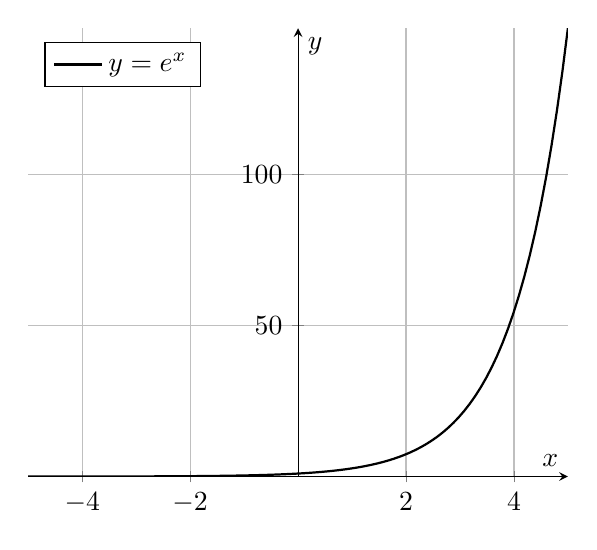
\begin{tikzpicture}
		        \begin{axis}[
			    axis lines = middle,
			    xlabel = $x$,
			    ylabel = {$y$},
			    domain=-5:5, % 定义x的区间
			    samples=100, % 采样点数量
			    grid = major, % 显示主网格线
			    legend pos=north west, % 图中方框的位置
			    ]
			    \addplot [
			        color=black,
			        thick,
			    ]{exp(x)};
			    \addlegendentry{$y = e^x$} 
		        \end{axis}
	        \end{tikzpicture}
            \end{center}
            {\fangsong 在这部分,需要利用指数函数的极限性质来求解问题。不难发现,$ \lim\limits_{x \to +\infty} e^x = +\infty$,
            $ \lim\limits_{x \to -\infty} e^x = 0$。}
            
            \quad
            
            (1) 设$f(x)=\lim\limits_{x \to \infty} \frac{x^{2n+1} + (a-1)x^n - 1}{x^2n -ax^n - 1}~(a\neq 0)$:
            
            \qquad (i) 求$f(x)$;

            \qquad (ii) 当$x \geqslant 0$时,若$f(x)$在连续,求$a$的值.

            (2)设$f(x) = \frac{x^{2} e^{n(x+1)} +ax + b}{e^{n(x+1) + 1}}$,试确定 $a,b$使得$f(x)$在处处可导,并 $f'(x)$.

            \begin{mdframed}
            (1) \textbf{解:}
            
            \end{mdframed}

            \begin{mdframed}
            (2) \textbf{解:}

            \end{mdframed}

    \section{微分中值定理与导数的应用}
        \subsection{微分中值定理}
            \subsubsection{罗尔定理}
            若函数$f(x)$满足:在$[a,b]$上连续;在$(a,b)$内可导;$f(a) = f(b)$;则在$(a,b)$内至少存在一个$\xi \in (a,b)$,使得$f'(\xi) = 0$.

            \subsubsection{拉格朗日中值定理}
            如果函数$f(x)$在闭区间$[a,b]$上连续,在开区间在$(a,b)$内可导,则至少存在一点$\xi \in (a,b)$,使得
            $$f'(\xi)=\frac{f(b)-f(a)}{b-a}$$

            \subsubsection{柯西中值定理}
            如果函数$f(x)$与$g(x)$在闭区间$[a,b]$上连续,在开区间在$(a,b)$内可导,并且在$(a,b)$内可
            $g'(x) \neq 0$,则至少存在一点$\xi \in (a,b)$,使得
            $$\frac{f(b)-f(a)}{g(b)-g(a)} = \frac{f'(\xi)}{g'(\xi)}$$
            
            \subsubsection{微分中值定理证明题}
            (1)设实数$a_0,a_1,\cdots,a_n$满足$a_0+\frac{a_1}{2}+\frac{a_2}{3}+\cdots+\frac{a_n}{n+1}=0$
            ,证明:方程$a_0+a_1 x+a_2 x^2+\cdots+a_n x^n=0$在$(0,1)$至少有一个实根.

            \begin{mdframed}
            (1) \textbf{解:}
            本题考察注意力。

            注意到当我们设$F(x) = a_0 x + \frac{a_1}{2} x^2 + \cdots + \frac{a_n}{n+1} x^{n+1}$时,$F(1) = 0$.

            同时$F'(x) = a_0 + a_1 x + a_2 x^2 + \cdots + a_n x^n$就是我们要证明的函数.

            所以由罗尔定理,对于$[0,1]$连续,$(0,1)$可导的$F(x)$,有$F(0)=F(1)$,则至少存在一个$\xi \in (0,1)$使得$F'(\xi) = 0$.

            \end{mdframed}
        \subsection{洛必达法则}
            洛必达法则用于求解不定式极限,主要适用于$\frac{0}{0}$和$\frac{\infty}{\infty}$两种类型的不定式。

            \textbf{定理:}
            设函数$f(x)$和$g(x)$在$x=a$的某邻域内可导,且$g'(x) \neq 0$,如果
            $$\lim\limits_{x \to a} f(x) = \lim\limits_{x \to a} g(x) = 0 \quad \text{或} \quad \lim\limits_{x \to a} f(x) = \lim\limits_{x \to a} g(x) = \pm \infty,$$
            则
            $$\lim\limits_{x \to a} \frac{f(x)}{g(x)} = \lim\limits_{x \to a} \frac{f'(x)}{g'(x)},$$

            \textbf{例题:}
            \begin{itemize}
                \item 例1:求$\lim\limits_{x \to 0} \frac{\sin x}{x}$。
                \begin{mdframed}
                \textbf{解:}
                直接应用洛必达法则:
                $$\lim\limits_{x \to 0} \frac{\sin x}{x} = \lim\limits_{x \to 0} \frac{\cos x}{1} = \cos 0 = 1.$$
                \end{mdframed}

                \item 例2:求$\lim\limits_{x \to \infty} \frac{e^x}{x^2}$。
                \begin{mdframed}
                \textbf{解:}
                直接应用洛必达法则:
                $$\lim\limits_{x \to \infty} \frac{e^x}{x^2} = \lim\limits_{x \to \infty} \frac{e^x}{2x} = \lim\limits_{x \to \infty} \frac{e^x}{2} = \infty.$$
                \end{mdframed}
            \end{itemize}

        \subsection{泰勒公式及其应用}
            \subsubsection{泰勒公式}
            \textbf{定理1:}
            \begin{mdframed}
            $f(x) = f(a) + f'(a)(x-a) + \frac{f''(a)}{2!}(x-a)^2 + \cdots + \frac{f^{(n)}(a)}{n!}(x-a)^n + o((x-a)^n)$
            \end{mdframed}
            其中$R_n(x) = o((x-a)^n)$称为皮亚诺余项.          
            
            \textbf{定理2:}
            \begin{mdframed}
            $f(x) = f(a) + f'(a)(x-a) + \frac{f''(a)}{2!}(x-a)^2 + \cdots + \frac{f^{(n)}(a)}{n!}(x-a)^n + R_n(x)$      
            \end{mdframed}          
            其中$R_n(x)=\frac{f^{(n+1)} (\xi)}{(n+1)!}(x-a)^{n+1}$称为拉格朗日型余项.

            \subsubsection{麦克劳林公式}
            \begin{itemize}
                \item $e^x = 1 + x + \frac{x^2}{2!} + \frac{x^3}{3!} + \cdots + \frac{x^n}{n!} + o(x^n)$
                \item $\sin x = x - \frac{x^3}{3!} + \frac{x^5}{5!} - \cdots + (-1)^n \frac{x^{2n+1}}{(2n+1)!} + o(x^{2n+1})$
                \item $\cos x = 1 - \frac{x^2}{2!} + \frac{x^4}{4!} - \cdots + (-1)^n \frac{x^{2n}}{(2n)!} + o(x^{2n})$
                \item $\tan x = x + \frac{x^3}{3} + \frac{2x^5}{15} + \cdots + \frac{B_{2n} x^{2n-1}}{(2n)!} + o(x^{2n-1})$
                \item $\ln(1+x) = x - \frac{x^2}{2} + \frac{x^3}{3} - \cdots + (-1)^{n-1} \frac{x^n}{n} + o(x^n)$
                \item $(1+x)^\alpha = 1 + \alpha x + \frac{\alpha(\alpha-1)}{2!}x^2 + \cdots + \frac{\alpha(\alpha-1)\cdots(\alpha-n+1)}{n!}x^n + o(x^n)$
                \item $\frac{1}{1-x} = 1 + x + x^2 + \cdots + x^n + o(x^n)$
            \end{itemize}
        
        \subsection{函数的性质}
            \subsubsection{函数的单调性}
            \textbf{定理:}
            \begin{mdframed}
            若函数$f(x)$在$[a,b]$上连续,在$(a,b)$内可导,则:
            \begin{itemize}
                \item 若$f'(x) > 0$,则$f(x)$在$(a,b)$上单调递增;
                \item 若$f'(x) < 0$,则$f(x)$在$(a,b)$上单调递减;
                \item 若$f'(x) = 0$,则$f(x)$在$(a,b)$上为常数函数.
            \end{itemize}
            \end{mdframed}

            \subsubsection{函数的极值}
            \textbf{定理:}
            \begin{mdframed}
            若函数$f(x)$在$x_0$处可导,且$f'(x_0) = 0$,则:
            \begin{itemize}
                \item 若$f'(x)$在$x_0$两侧异号,则$f(x)$在$x_0$处取极值.
                \item 若$f'(x)$在$x_0$两侧同号,则$f(x)$在$x_0$处无极值.
            \end{itemize}
            \end{mdframed}

            \textbf{极值的第一充分条件:}
            \begin{mdframed}
            若函数$f(x)$在$x_0$处连续,在$x_0$的去心邻域$\delta$内可导,且$x_0$是$f(x)$的驻点或不可导点,则:
            \begin{itemize}
                \item 当$x \in (x_0 - \delta , x_0)$时,$f'(x) > 0$;
                当$x \in (x_0  , x_0 + \delta)$时,$f'(x) < 0$;则$f(x)$在$x_0$处取极大值.
                \item 当$x \in (x_0 - \delta , x_0)$时,$f'(x) < 0$;
                当$x \in (x_0  , x_0 + \delta)$时,$f'(x) > 0$;则$f(x)$在$x_0$处取极小值.
                \item 当$x \in (x_0 - \delta , x_0) \cup (x_0  , x_0 + \delta)$时,$f'(x) > 0$或$f'(x) < 0$,
                则$f(x)$在$x_0$处无极值.
            \end{itemize}
            \end{mdframed}

            \textbf{极值的第二充分条件:}
            \begin{mdframed}
            若函数$f(x)$在$x_0$处连续,在$x_0$的去心邻域$\delta$内二阶可导,且$f'(x_0) = 0$,$f''(x_0) \neq 0$,则:
            \begin{itemize}
                \item 当$f''(x_0) > 0$时,$f(x)$在$x_0$处取极小值;
                \item 当$f''(x_0) < 0$时,$f(x)$在$x_0$处取极大值.
            \end{itemize}
            \end{mdframed}

            \subsubsection{函数的凹凸性}
            \textbf{凹凸性的定义:}
            \begin{mdframed}
            若函数$f(x)$在$(a,b)$上连续,对于任意$x_0 \in (a,b)$,都有:
            $$f(x) > f(x_0) + f'(x_0) (x-x_0)$$
            则称$f(x)$在$(a,b)$上凹函数;
            若函数$f(x)$在$(a,b)$上连续,对于任意$x_0 \in (a,b)$,都有:
            $$f(x) < f(x_0) + f'(x_0) (x-x_0)$$
            则称$f(x)$在$(a,b)$上凸函数.
            \end{mdframed}

            \textbf{凹凸性的充分条件:}
            \begin{mdframed}
            若函数$f(x)$在$(a,b)$上二阶可导,则:
            \begin{itemize}
                \item 若$f''(x) > 0$,则$f(x)$在$(a,b)$上凹函数;
                \item 若$f''(x) < 0$,则$f(x)$在$(a,b)$上凸函数.
            \end{itemize}
            \end{mdframed}

            \textbf{定理:}
            \begin{mdframed}
            若函数$f(x)$在$(a,b)$上连续,在$(a,b)$内二阶可导:
            
            若对于$(a,b)$内任意两点$x_1,x_2$,有
            $$f(\frac{x_1+x_2}{2}) < \frac{f(x_1)+f(x_2)}{2}$$
            则称$f(x)$在$(a,b)$上凹函数;
            
            若有
            $$f(\frac{x_1+x_2}{2}) > \frac{f(x_1)+f(x_2)}{2}$$
            则称$f(x)$在$(a,b)$上凸函数.
            \end{mdframed}

            在这里有扩展定理,即著名的 \textbf{Jensen不等式}:
            \begin{mdframed}
            若函数$f(x)$在$(a,b)$上连续,在$(a,b)$内二阶可导,且$f''(x) > 0$,\\
            则对于任意$x_1,x_2,\cdots,x_n \in (a,b)$,以及任意$n$个正数$\lambda_1,\lambda_2,\cdots,\lambda_n$,满足$\sum\limits_{i=1}^{n} \lambda_i = 1$,有
            $$f(\sum\limits_{i=1}^{n} \lambda_i x_i) < \sum\limits_{i=1}^{n} \lambda_i f(x_i)$$

            同理,若$f''(x) < 0$,则有
            $$f(\sum\limits_{i=1}^{n} \lambda_i x_i) > \sum\limits_{i=1}^{n} \lambda_i f(x_i)$$

            还有一种易读的形式
            
            对于任意凹函数,都有:
            $$f(\frac{x_1 + x_2 + \cdots + x_n}{n}) > \frac{f(x_1) + f(x_2) + \cdots + f(x_n)}{n}$$

            对于任意凸函数,都有:
            $$f(\frac{x_1 + x_2 + \cdots + x_n}{n}) < \frac{f(x_1) + f(x_2) + \cdots + f(x_n)}{n}$$

            \end{mdframed}

            \subsubsection{函数的拐点}
            \textbf{拐点的定义:}
            \begin{mdframed}
            若函数$f(x)$在$x_0$处连续,在$x_0$的去心邻域$\delta$内二阶可导,且$f'(x_0) = 0$,则:
            \begin{itemize}
                \item 当$f''(x_0)$在$x_0$两侧异号,则$f(x)$在$x_0$处取拐点.
                \item 当$f''(x_0)$在$x_0$两侧同号,则$f(x)$在$x_0$处无拐点.
                \item 当$f''(x_0)$在$x_0$两侧为零,则$f(x)$在$x_0$处可能有拐点,也可能无拐点.
            \end{itemize}
            \end{mdframed}

            \subsubsection{函数的渐近线}
            \textbf{垂直渐近线:}
            \begin{mdframed}
            若函数$f(x)$在$x_0$处连续,在$x_0$的去心邻域$\delta$内可导,且$\lim\limits_{x \to x_0} f'(x) = \pm \infty$,则直线$x = x_0$称为$f(x)$的垂直渐近线.
            \end{mdframed}

            \textbf{水平渐近线:}
            \begin{mdframed}
            若$\lim\limits_{x \to \infty} f(x) = A$,则直线$y = A$称为$f(x)$的水平渐近线.
            \end{mdframed}

            \textbf{斜渐近线:}
            \begin{mdframed}
            若$\lim\limits_{x \to \infty} [f(x) - (ax+b)] = 0$,则直线$y = ax+b$称为$f(x)$的斜渐近线.  
            \end{mdframed}

        \subsection{曲线的曲率}
            \textbf{曲率的定义:}
            \begin{mdframed}
            设曲线$y=f(x)$在点$M(x_0,y_0)$处可导,且$f'(x)$在$x_0$的某邻域内连续,且$f'(x) \neq 0$,则曲线$y=f(x)$在点$M(x_0,y_0)$处的曲率为
            $$K = \frac{|f''(x_0)|}{[1+(f'(x_0))^2]^{\frac{3}{2}}}$$
            \end{mdframed}
            
            \textbf{弧微分:}
            \begin{mdframed}
            设曲线$y=f(x)$在点$M(x_0,y_0)$处可导,且$f'(x)$在$x_0$的某邻域内连续,且$f'(x) \neq 0$,则曲线$y=f(x)$在点$M(x_0,y_0)$处的弧微分为
            $$ds = \sqrt{1+(f'(x))^2}dx$$
            \end{mdframed}

            \textbf{曲率圆:}
            \begin{mdframed}
            设曲线$y=f(x)$在点$M(x_0,y_0)$处可导,且$f'(x)$在$x_0$的某邻域内连续,且$f'(x) \neq 0$,则曲线$y=f(x)$在点$M(x_0,y_0)$处的曲率圆为
            $$\begin{cases}
                x = x_0 + \frac{1}{K} \cos \theta\\
                y = y_0 + \frac{1}{K} \sin \theta
            \end{cases}$$

            其中$\theta$为曲线$y=f(x)$在点$M(x_0,y_0)$处的切线与$x$轴的夹角.

            曲率半径为$R = \frac{1}{K}$.

            曲率中心$(\xi,\eta)$为$$\begin{cases}
                \xi = x_0 - \frac{f'(x_0)[1+(f'(x_0))^2]}{f'(x_0)}\\
                \eta = y_0 + \frac{1+(f'(x_0))^2}{f''(x_0)}
            \end{cases}$$

            \end{mdframed}

        \subsection{典型题目}
            \subsubsection{抽象函数的洛必达应用}
            1. 设$f(x)$在$(-\infty , +\infty)$内具有二阶导数,且$f(0)=f'(0)=0$,\\试求
            $g(x)=\begin{cases}
                \frac{f(x)}{x} & x \neq 0\\
                0 & x = 0
            \end{cases}$
            的导数。

            2.设$f(x)$在$a$邻域可导,且在$a$处二阶可导,求$
            \lim\limits_{h \to 0}\frac{f(a+h)+f(a-h)-2f(a)}{h^2}$

            \begin{mdframed}
            1. \textbf{解:}
            当$x = 0$时,$g'(0) = \lim\limits_{x \to 0} \frac{g(x) - g(0)}{x} = 
            \lim\limits_{x \to 0} \frac{f(x)}{x^2} = \lim\limits_{x \to 0} \frac{f'(x)}{2x}$(洛必达法则)\\
            $= \lim\limits_{x \to 0} \frac{f'(x)}{2x} = \lim\limits_{x \to 0} $.
            \end{mdframed}

\end{document}